\documentclass[a4paper,twoside]{article}
\usepackage{blindtext}  
\usepackage{geometry}

% Chinese support
\usepackage[UTF8, scheme = plain]{ctex}

% Page margin layout
\geometry{left=2.3cm,right=2cm,top=2.5cm,bottom=2.0cm}


\usepackage{listings}
\usepackage{xcolor}
\usepackage{geometry}
\usepackage{amsmath}
\usepackage{float}
\usepackage{hyperref}

\usepackage{graphics}
\usepackage{graphicx}
\usepackage{subcaption}
\usepackage{epsfig}
\usepackage{float}

\usepackage{algorithm}
\usepackage[noend]{algpseudocode}

\usepackage{booktabs}
\usepackage{threeparttable}
\usepackage{longtable}
\usepackage{tikz}
\usepackage{multicol}
\usepackage{pgfplots}
\pgfplotsset{compat=1.9}
\pgfplotsset{
    myplotstyle/.style={
    legend style={draw=none, font=\small},
    legend cell align=left,
    legend pos=north east,
    ylabel style={align=center, font=\bfseries\boldmath},
    xlabel style={align=center, font=\bfseries\boldmath},
    x tick label style={font=\bfseries\boldmath},
    y tick label style={font=\bfseries\boldmath},
    scaled ticks=false,
    every axis plot/.append style={thick},
    },
}

% cite package, to clean up citations in the main text. Do not remove.
\usepackage{cite}

\usepackage{color,xcolor}

%% The amssymb package provides various useful mathematical symbols
\usepackage{amssymb}
%% The amsthm package provides extended theorem environments
\usepackage{amsthm}
\usepackage{amsfonts}
\usepackage{enumerate}
\usepackage{enumitem}
\usepackage{listings}
\usepackage{minted}


\usepackage{indentfirst}
\setlength{\parindent}{2em} % Make two letter space in the first paragraph
\usepackage{setspace}
\linespread{1.5} % Line spacing setting
\usepackage{siunitx}
\setlength{\parskip}{0.5em} % Paragraph spacing setting

% \usepackage[contents =22920202204622, scale = 10, color = black, angle = 50, opacity = .10]{background}

\renewcommand{\figurename}{图}
\renewcommand{\listingscaption}{代码}
\renewcommand{\tablename}{表格}
\renewcommand{\contentsname}{目录}
\floatname{algorithm}{算法}

\graphicspath{ {images/} }

%%%%%%%%%%%%%
\newcommand{\StudentNumber}{22920202204622}  % Fill your student number here
\newcommand{\StudentName}{熊恪峥}  % Replace your name here
\newcommand{\PaperTitle}{实验(三)欧拉操作系统内核操作}  % Change your paper title here
\newcommand{\PaperType}{操作系统实验报告} % Replace the type of your report here
\newcommand{\Date}{2023年5月19日}
\newcommand{\College}{信息学院}
\newcommand{\CourseName}{操作系统}
%%%%%%%%%%%%%

%% Page header and footer setting
\usepackage{fancyhdr}
\usepackage{lastpage}
\pagestyle{fancy}
\fancyhf{}
% This requires the document to be twoside
\fancyhead[LO]{\texttt{\StudentName }}
\fancyhead[LE]{\texttt{\StudentNumber}}
\fancyhead[C]{\texttt{\PaperTitle }}
\fancyhead[R]{\texttt{第{\thepage}页,共\pageref*{LastPage}页}}


\title{\PaperTitle}
\author{\StudentName}
\date{\Date}

\algnewcommand\algorithmicinput{\textbf{Input:}}
\algnewcommand\algorithmicoutput{\textbf{Output:}}
\algnewcommand\Input{\item[\algorithmicinput]}%
\algnewcommand\Output{\item[\algorithmicoutput]}%

\usetikzlibrary{positioning, shapes.geometric,arrows,automata}

\tikzstyle{startstop} = [rectangle, rounded corners, minimum width=3cm, minimum height=1cm, text centered, draw=black, fill=red!30]
\tikzstyle{io} = [trapezium, trapezium left angle=70, trapezium right angle=110, minimum width=3cm, minimum height=1cm, text centered, draw=black, fill=blue!30]
\tikzstyle{process} = [rectangle, minimum width=3cm, minimum height=1cm, text centered, draw=black, fill=green!30]
\tikzstyle{decision} = [diamond, minimum width=3cm, minimum height=1cm, text centered, draw=black, fill=yellow!30]
\tikzstyle{arrow} = [thick,->,>=stealth]

\begin{document}
	
%%%%%%%%%%%%%%%%%%%%%%%%%%%%%%%%%%%%%%%%%%%%
\makeatletter % change default title style
\renewcommand*\maketitle{%
	\begin{center} 
		\bfseries  % title 
		{\LARGE \@title \par}  % LARGE typesetting
		\vskip 1em  %  margin 1em
		{\global\let\author\@empty}  % no author information
		{\global\let\date\@empty}  % no date
		\thispagestyle{empty}   %  empty page style
	\end{center}%
	\setcounter{footnote}{0}%
}
\makeatother
%%%%%%%%%%%%%%%%%%%%%%%%%%%%%%%%%%%%%%%%%%%%
	
	
\thispagestyle{empty}

\vspace*{1cm}

\begin{figure}[htb]
	\centering
	
\includegraphics[width=4.0cm]{logo.png}
\end{figure}

\vspace*{1cm}

\begin{center}
	\Huge{\textbf{\PaperType}}
	
	\Large{\PaperTitle}
\end{center}

\vspace*{1cm}

\begin{table}[H]
	\centering	
	\begin{Large}
		\renewcommand{\arraystretch}{1.5}
		\begin{tabular}{p{3cm} p{5cm}<{\centering}}
			姓\qquad 名 & \StudentName  \\
			\hline
			学\qquad号 & \StudentNumber \\
			\hline
			日\qquad期 & \Date  \\
			\hline
			学\qquad院 & \College  \\
			\hline
			课程名称 & \CourseName  \\
			\hline
		\end{tabular}
	\end{Large}
\end{table}

\newpage

\title{
	\Large{\textcolor{black}{\PaperTitle}}
}

\maketitle
	
\tableofcontents
 
\newpage
\setcounter{page}{1}

\begin{spacing}{1.2}

\section{实验内容}

本实验通过安装openEuler操作系统、编译安装openEuler操作系统新内核以及简单的内核模块编程任务操作带领大家了解操作系统及内核编程。  

\section{目的}

\begin{enumerate}
	\item 学习掌握如何安装操作系统
	\item 学习掌握如何编译操作系统内核
	\item 了解内核模块编程
\end{enumerate}

\section{编译和安装}

首先,备份boot目录和版本信息,如图~\ref*{fig:backup}
\begin{figure}[H]
	\centering
	\caption{备份}
	\label{fig:backup}
	\begin{subfigure}{0.45\textwidth}
		\centering
		\includegraphics*[width=0.9\textwidth]{1.png}
	\end{subfigure}
	\begin{subfigure}{0.45\textwidth}
		\centering
		\includegraphics*[width=0.9\textwidth]{2.png}
	\end{subfigure}
\end{figure}
然后获取内核源码并解压,如图~\ref{fig:code}
\begin{figure}[H]
	\centering
	\caption{获取内核源码并解压}
	\label{fig:code}
	\begin{subfigure}{0.45\textwidth}
		\centering
		\includegraphics*[width=0.9\textwidth]{3.png}
	\end{subfigure}
	\begin{subfigure}{0.45\textwidth}
		\centering
		\includegraphics*[width=0.9\textwidth]{4.png}
	\end{subfigure}
\end{figure}
然后,把源码目录命名为\texttt{kernel}。如图~\ref{fig:rename}
\begin{figure}[H]
	\centering
	\caption{把源码目录命名为\texttt{kernel}}
	\label{fig:rename}
	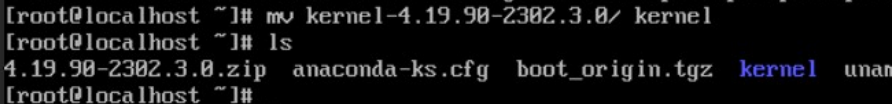
\includegraphics[width=0.4\textwidth]{5.png}
\end{figure}
接着,进入源码目录,配置内核并编译,如图~\ref{fig:config}
\begin{figure}[H]
	\centering
	\caption{配置内核并编译}
	\label{fig:config}
	\begin{subfigure}{0.45\textwidth}
		\centering
		\includegraphics*[width=0.9\textwidth]{6.png}
	\end{subfigure}
	\begin{subfigure}{0.45\textwidth}
		\centering
		\includegraphics*[width=0.9\textwidth]{7.png}
	\end{subfigure}
\end{figure}
最后,进行安装,如图~\ref{fig:install}。
\begin{figure}[H]
	\centering
	\caption{配置内核并编译}
	\label{fig:install}
	\begin{subfigure}{0.45\textwidth}
		\centering
		\includegraphics*[width=0.9\textwidth]{8.png}
	\end{subfigure}
	\begin{subfigure}{0.45\textwidth}
		\centering
		\includegraphics*[width=0.9\textwidth]{9.png}
	\end{subfigure}
\end{figure}
重启之后检查内核版本,并在grub中设置默认内核,如图~\ref{fig:fin}
\begin{figure}[H]
	\centering
	\caption{使用新内核}
	\label{fig:fin}
	\begin{subfigure}{0.45\textwidth}
		\centering
		\includegraphics*[width=0.9\textwidth]{10.png}
	\end{subfigure}
	\begin{subfigure}{0.45\textwidth}
		\centering
		\includegraphics*[width=0.9\textwidth]{11.png}
	\end{subfigure}
\end{figure}


\section{任务一}

查找相关资料,解释\texttt{hello\_world.c}文件中以下代码的含义和作用:
\begin{enumerate}
	\item MODULE\_LICENSE:在Linux内核文档有如下表述:
	\begin{quotation}
		The sole purpose of this tag is to provide sufficient information whether the module is free software or proprietary for the kernel module loader and for user space tools.
	\end{quotation}
	即这个tag提供了以便内核模块加载器和用户空间工具判断模块是自由软件还是专有软件的信息。
	\item module\_param:是用于定义模块参数的宏,三个参数分别为变量名、类型、权限。
	\item MODULE\_PARM\_DESC:用于定义模块参数的描述的宏。描述会在使用\texttt{modinfo}命令时显示出来
	\item module\_init: 用于通知内核初始化模块的时候, 要使用哪个函数进行初始化。
	\item module\_exit: 用于告诉内核,当卸载模块时,需要调用哪个函数。
	\item \_\_init:用于将函数放在可执行文件的init段中,将在初始化时被执行。
	\item \_\_exit:将函数放在exit段中,在模块卸载阶段执行。
\end{enumerate}

内容出处:
\begin{enumerate}
	\item \url{https://tldp.org/LDP/lkmpg/2.6/html/x323.html}
	\item \url{https://www.kernel.org/doc/html/latest/process/license-rules.html#id1}
\end{enumerate}

\section{任务二}

请参考hello\_world.c和Makefile文件,在右侧代码文件区域编写hello\_magic\_student.c和 Makefile文件,完成以下任务:

\begin{enumerate}
	\item 在hello\_magic\_student.c文件中定义函数 hello\_student(…),该函数包含3个参数:id, name, age,分别代表学号、姓名和年龄,并通过printk输出:
	\begin{minted}{python3}
My name is ${name}, student id is ${id}. I am ${age} years old.
	\end{minted}
	\item 在hello\_magic\_student.c文件中定义函数 my\_magic\_number(…),该函数包含2个参数:id和age,分别代表学号和年龄。请你在该函数里将学号的每一位数字相加后再与年龄求和,将求和结果的个位数作为magic\_number,并使用printk输出:
	\begin{minted}{python3}
My magic number is ${magic_number}.
	\end{minted}
\end{enumerate}

完成hello\_magic\_student.c文件的编写后,系统会自动保存。参考hello\_world模块的Makefile并适当调整,在加载内核时提供学号、姓名和年龄,通过dmesg命令查看printk的输出。  

首先,在文件开始处的三个参数定义进行修改,写入自己的姓名学号年龄:
\begin{minted}{c}
	/*id*/
static char* id = "22920202204622";
module_param(id, charp, 0644);
MODULE_PARM_DESC(id, "char* param\n");

/*name*/
static char* name = "KeZheng Xiong";
module_param(name, charp, 0644);
MODULE_PARM_DESC(name, "char* param\n");

/*age*/
static int age = 21;
module_param(age, int, 0644);
MODULE_PARM_DESC(age, "int param\n");
\end{minted}

然后依题意实现两个函数即可。前者直接调用\texttt{printk}输出,该函数的使用方式与\texttt{printf}一致。后者遍历学号、转化为整数并按规则计算:
\begin{minted}{c}
void hello_student(char* id,char *name,int age)
{
    printk("My name is %s, student id is %s. I am %d years old.",name,id,age);
}
void my_magic_number(char* id,int age)
{
    int ret=0;
    char *p=id;
    while(*p){
        ret+=(*p++ -'0');
    }
    ret+=age;
    printk("My magic number is %d.",ret%10);
} 
\end{minted}

首先,编译该模块,输出信息如图~\ref{fig:cmp},无错误后安装模块。
\begin{figure}[H]
	\centering
	\caption{编译模块}
	\label{fig:cmp}
	\includegraphics*[width=0.6\textwidth]{build.png}
\end{figure}
然后,使用\texttt{insmod}安装内核模块,然后等待一段时间,使用\texttt{dmesg}查看输出,如图~\ref{fig:out}。
\begin{figure}[H]
	\centering
	\caption{输出信息}
	\label{fig:out}
	\includegraphics*[width=0.6\textwidth]{res.png}
\end{figure}
可见该实现正确地输出了相关信息。计算结果也是正确的(按照规则求和得56,个位为6)。

\section{实验总结}

在本次实验中,我编译并运行了Linux内核。在自行编译运行的基础上,我实现了一个简单的
内核模块。了解了Linux内核模块的编程并进行了实际体验。
在实验中,我对Linux内核编程的细节有了更多把握,并且注意了Makefile中需要使用Tab而非空格,否则会出现错误。


\end{spacing}

\end{document}